151. \begin{figure}[ht!]
\center{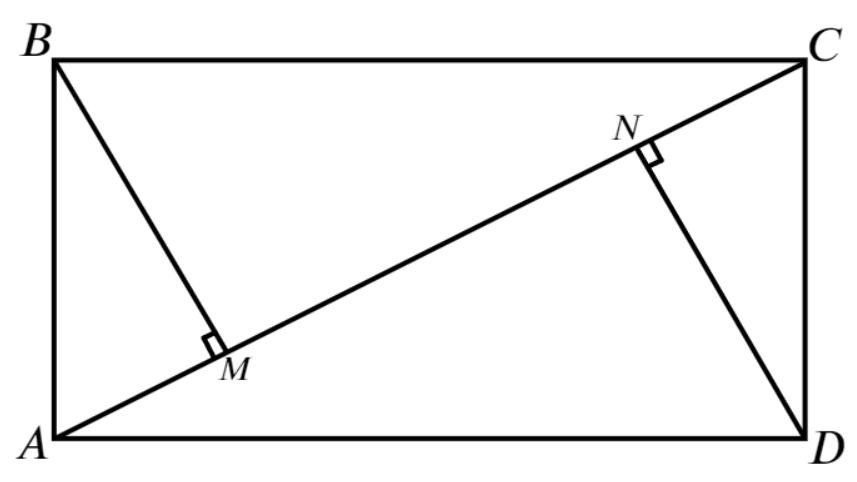
\includegraphics[scale=0.35]{g9-151.png}}
\end{figure}\\
Пусть $AM=CN=x$ (эти отрезки равны так как по катету и гипотенузе равны треугольники $ABM$ и $CDN$). Треугольники $AND$ и $DNC$ подобны по двум  углам ($\angle AND=\angle DNC=90^\circ,\ \angle NDC=90^\circ-\angle ACD=\angle CAD).$ Тогда $\cfrac{AN}{ND}=\cfrac{ND}{CN},\ \cfrac{x+15}{4}=\cfrac{4}{x},\ x^2+15x=16,\ x^2+15x-16=0,\
(x-1)(x+16)=0,\ x=1.$ Тогда $S_{ABCD}=2S_{\Delta ACD}=2\cdot\cfrac{1}{2}\cdot4\cdot17=68.$\newpage\noindent
